\documentclass{article}
\usepackage[utf8]{inputenc}

\title{NTIN066 - Fibonacci heap}
\author{Thuong-Hai Pham}
\date{November 2017}

\usepackage{graphicx}

\begin{document}

\maketitle

\section{Random test vs. Biased test}

\begin{figure}[h!]
\centering
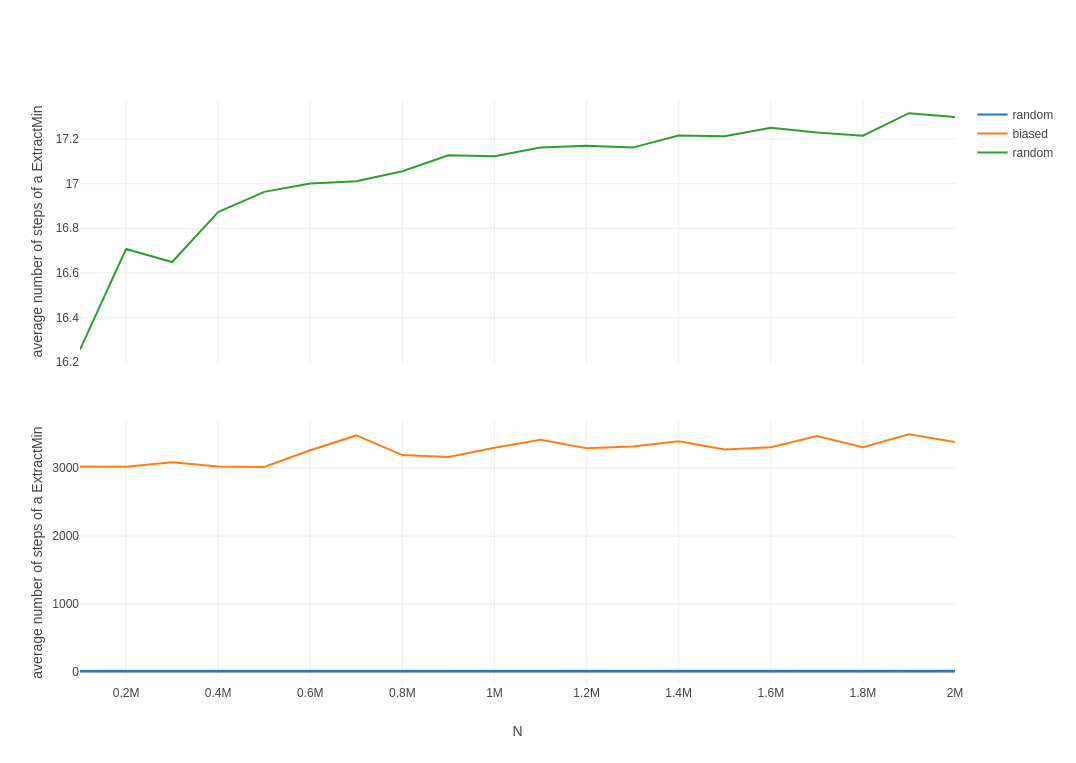
\includegraphics[width=\textwidth]{NTIN066-fibheap-plot3}
\caption{Random and Biased test result}
\label{fig:plot3}
\end{figure}

In Figure \ref{fig:plot3}, the random test (green and blue lines) illustrates the amortized complexity of ExtractMin (DeleteMin) operation is $O(log(n))$.

The difference between random and biased test is that the number of delete operations in random $nr\_del=\frac{n}{1.6}$, while in biased test, $nr\_del'=\frac{n}{1000+1.6}$, i.e. 1000 times smaller than in random test. Yet the problem is that the number of decrease operations changes from $nr\_dec=5.25n$ (random) to $nr\_dec'\approx 2n$ (biased). Let us make an approximation in a naive way that the number of steps in an ExtractMin operation is the number of nodes created by decrease operation before it and each decrease operation only puts one node into the tree list, then the average number of steps in biased test is $\approx 238$ times larger than in random test, i.e. $n$ with average of 17 steps in random test will have $\approx 4000$ steps in biased. However, the average number of steps also depends on the order of the min node and one decrease operation does not cut only one node. Hence, it explains the result in Figure \ref{fig:plot3}.

\section{Proper and Naive Fibonacci heap}

The special test case tricks the naive Fibonacci heap into one particular scenario:

After a finite number of operations, because the lack of cascading cut, naive Fibonacci heap has created a heap of which its $k$ trees have only zero-order children. For example, with $N=13$, $k=4$:

\begin{figure}[h!]
\centering
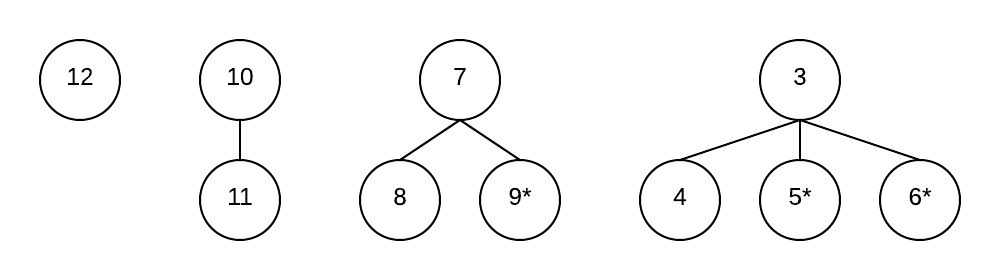
\includegraphics[width=\textwidth]{special-naive}
\caption{Naive Fibonacci heap}
\label{fig:naive}
\end{figure}

From this point onward, the generator only inserts two node with 1 and 2 key, following by two delete operations. The first delete operation deletes node with key = 1, the consolidation procedure links all the trees in Figure \ref{fig:naive} as the child of node 2, i.e. number of steps = k = 4. Consequently, the second delete operation deletes node 2, brings all those k trees back to the tree list, i.e. number of steps = k = 4. This sequence of operations is repeated throughout the test case. Hence the average number of steps of ExtractMin operations $\approx k\approx 4$ in our case of $N=13$.

To build the scenario described above, the generator needs at least $1+2+...+k = \frac{k(k+1)}{2}$ nodes, plus some dummy nodes. To be precise, the heapgen generator needs $N=3+\frac{k(k+1)}{2}$. Hence, the average number of steps of ExtractMin operations in this special test with naive Fibonacci heap is $\Theta(\sqrt{N})$.

In contrast, with cascading cut, proper Fibonacci heap is not tricked into the scenario above. The trees in proper Fibonacci heap, after a finite number of operations of this special test, will have high order, hence, will not interact with the dummy nodes (newly inserted nodes e.g. node 1 and 2). For examples, the green line in Figure \ref{fig:plot2} shows that for most test cases, the trees will have order larger than 2, hence node 1 and 2 will not be joined with these trees  as in Naive heap. Therefore, the average number of steps is 0.

However, please be noted that the order in the tree list and among children of a node is arbitrary, and the special test generator is not well built for this. That leads to different results for various implementation of inserting a node into the children list or a tree into the tree list. For example, the green and blue lines in Figure \ref{fig:plot2} shows 2 different results when inserting to the left of the minHeap node (proper, green) and to the right (proper2, blue). This arbitrariness also leads to inserting existing node to the heap in this special test case. Nevertheless, in all implementations of the proper heap, after a finite small number of operations, the average steps is a small constant as all the trees are high-order and the dummy nodes can only interact with a limited number of trees or no tree at all. That illustrates the complexity of $\Theta(1)$ as in Figure \ref{fig:plot2}.


\begin{figure}[h!]
\centering
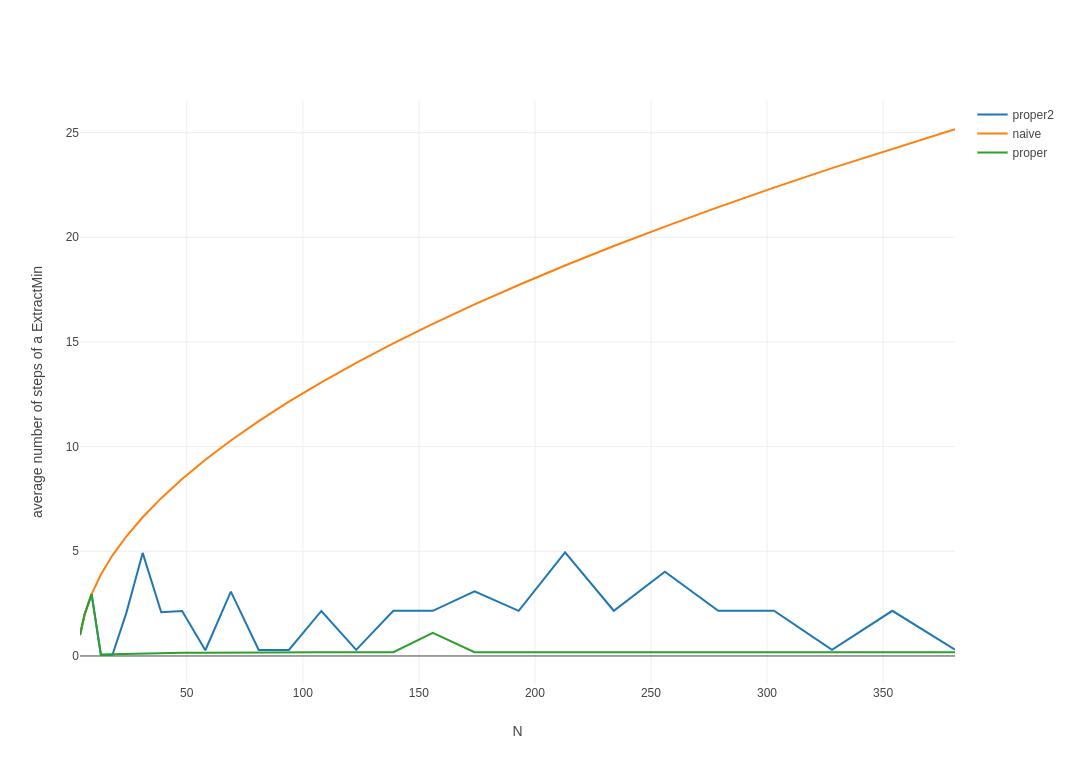
\includegraphics[width=\textwidth]{NTIN066-fibheap-plot2}
\caption{Special test result}
\label{fig:plot2}
\end{figure}


\end{document}
